\documentclass{article}
\usepackage{tikz}
\usepackage{pgfplots}
\usetikzlibrary{positioning}
\newdimen\nodeDist
\nodeDist=18mm

\usepackage{amsmath}
\usepackage{amssymb}
\usepackage{graphicx}
\usepackage{setspace}

\begin{document}

\title{Home Work 1 (CS6350)}
\author{Aishwarya Asesh (u1063384)}
\maketitle
\raggedright

\textbf {1: Decision Trees}
\\[10pt]
Question 1 : Represent the following Boolean functions as decision trees. (It is unnecessary to make the decision tree as small as possible; you can choose any root as you like. Use 1 for True and 0 for False. Also, note that an easy way to represent decision trees is as a series of if-then-else statements.)
\\[10pt]
Answer 1 :
\\[10pt]
(a) Decision Tree for: $\mathcal(x1 \lor x2) \land x3$
\\[10pt]
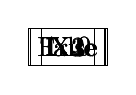
\begin{tikzpicture}[
    node/.style={%
      draw,
      rectangle,
    },
  ]

    \node [node] (A) {X3};
    \path (A) ++(-135:\nodeDist) node [node] (B) {X1};
    \path (A) ++(-45:\nodeDist) node [node] (C) {False};
    \path (B) ++(-135:\nodeDist) node [node] (D) {True};
    \path (B) ++(-45:\nodeDist) node [node] (E) {X2};
    \path (E) ++(-135:\nodeDist) node [node] (F) {True};
    \path (E) ++(-45:\nodeDist) node [node] (G) {False};


    \draw (A) -- (B) node [left,pos=0.25] {1}(A);
    \draw (A) -- (C) node [right,pos=0.25] {0}(A);
    \draw (B) -- (D) node [left,pos=0.25] {1}(A);
    \draw (B) -- (E) node [right,pos=0.25] {0}(A);
    \draw (E) -- (F) node [left,pos=0.25] {1}(A);
    \draw (E) -- (G) node [right,pos=0.25] {0}(A);
\end{tikzpicture}
\\[10pt]
(b) Decision Tree for: $\mathcal(x1 \land x2) xor (\neg x1 \lor x3)$
\\[10pt]
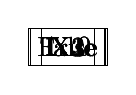
\begin{tikzpicture}[
    node/.style={%
      draw,
      rectangle,
    },
  ]

    \node [node] (A) {X1};
    \path (A) ++(-135:\nodeDist) node [node] (B) {X2};
    \path (A) ++(-45:\nodeDist) node [node] (C) {True};
    \path (B) ++(-135:\nodeDist) node [node] (D) {X3};
    \path (B) ++(-45:\nodeDist) node [node] (E) {X3};
    \path (D) ++(-115:\nodeDist) node [node] (F) {False};
    \path (D) ++(-65:\nodeDist) node [node] (G) {True};
    \path (E) ++(-115:\nodeDist) node [node] (I) {True};
    \path (E) ++(-65:\nodeDist) node [node] (J) {False};


    \draw (A) -- (B) node [left,pos=0.25] {1}(A);
    \draw (A) -- (C) node [right,pos=0.25] {0}(A);
    \draw (B) -- (D) node [left,pos=0.25] {1}(A);
    \draw (B) -- (E) node [right,pos=0.25] {0}(A);
    \draw (D) -- (F) node [left,pos=0.25] {1}(A);
    \draw (D) -- (G) node [right,pos=0.25] {0}(A);
    \draw (E) -- (I) node [left,pos=0.25] {1}(A);
    \draw (E) -- (J) node [right,pos=0.25] {0}(A);

\end{tikzpicture}
\\[10pt]
(c) Decision Tree for: 
\\The 2-of-3 function defined as follows: at least 2 of ${\{x1, x2, x3\}}$ should be true for the output to be true.
\\[10pt]
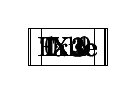
\begin{tikzpicture}[
    node/.style={%
      draw,
      rectangle,
    },
  ]

    \node [node] (A) {X1};
    \path (A) ++(-135:\nodeDist) node [node] (B) {X2};
    \path (A) ++(-45:\nodeDist) node [node] (C) {X3};
    \path (B) ++(-115:\nodeDist) node [node] (D) {True};
    \path (B) ++(-65:\nodeDist) node [node] (E) {X3};
    \path (C) ++(-115:\nodeDist) node [node] (F) {False};
    \path (C) ++(-65:\nodeDist) node [node] (G) {X2};
    \path (E) ++(-115:\nodeDist) node [node] (H) {True};
    \path (E) ++(-65:\nodeDist) node [node] (I) {False};
    \path (G) ++(-115:\nodeDist) node [node] (J) {True};
    \path (G) ++(-65:\nodeDist) node [node] (K) {False};


    \draw (A) -- (B) node [left,pos=0.25] {1}(A);
    \draw (A) -- (C) node [right,pos=0.25] {0}(A);
    \draw (B) -- (D) node [left,pos=0.25] {1}(A);
    \draw (B) -- (E) node [right,pos=0.25] {0}(A);
    \draw (C) -- (F) node [left,pos=0.25] {0}(A);
    \draw (C) -- (G) node [right,pos=0.25] {1}(A);
    \draw (E) -- (H) node [left,pos=0.25] {1}(A);
    \draw (E) -- (I) node [right,pos=0.25] {0}(A);
    \draw (G) -- (J) node [left,pos=0.25] {1}(A);
    \draw (G) -- (K) node [right,pos=0.25] {0}(A);


\end{tikzpicture}
\\[10pt]
Question 2 : When playing Pokemon Go, there is some chance that a Pokemon will be caught or it will escape. In the following question, build a decision tree to determine whether a Pokemon can be caught. There are four features:
\\(a) Berry (Yes or No) means whether a Razz Berry was used.
\\(b) Ball (Poke, Great, or Ultra) describes which kind of ball has been thrown.
\\(c) Color (Green, Yellow, or Red) stands for the diffculty level of catching this Pokemon.
\\(d) Type (Normal, Water, Flying, or Psychic) depicts the type of the Pokemon.
\\[10pt]
Answer 2 :
\\[10pt]
(a) Number of possible functions present there to map these four features to a Boolean decision $2^{16}$
\\[10pt]
(b) Entropy of the label = (-1) $((8/16) \log_{2} (8/16) + (8/16) \log_{2} (8/16))$  = 1.0
\\[10pt]
(c) Information Gain values for 4 attributes are as follows:
\\[10pt]
For attribute named "Berry"
\\
"Yes"
Entropy = (-1) $((6/7) \log_{2} (6/7) + (1/7) \log_{2} (1/7))$ = 0.591
\\
"No"
Entropy = (-1) $((2/9) \log_{2} (2/9) + (7/9) \log_{2} (7/9))$ = 0.763
\\
Total = (7/16)*0.591 + (9/16)*0.763 = 0.687
\\
Info Gain = 1 - 0.687
\\[10pt]
For attribute named "Ball"
\\
"Poke"
Entropy = (-1) $((1/6) \log_{2} (1/6) + (5/6) \log_{2} (5/6))$ = 0.649
\\
"Great"
Entropy = (-1) $((4/7) \log_{2} (4/7) + (3/7) \log_{2} (3/7))$ = 0.984
\\
"Ultra"
Entropy = (-1) $((3/3) \log_{2} (3/3))$ = 0.0
\\
Total = (6/16)*0.649 + (7/16)*0.984 = 0.673
\\
Info Gain = 1 - 0.673
\\[10pt]
For attribute named "Color"
\\
"Green"
Entropy = (-1) $((2/3) \log_{2} (2/3) + (1/3) \log_{2} (1/3))$ = 0.917
\\
"Yellow"
Entropy = (-1) $((3/7) \log_{2} (3/7) + (4/7) \log_{2} (4/7))$ = 0.984
\\
"Red"
Entropy = (-1) $((3/6) \log_{2} (3/6) + (3/6) \log_{2} (3/6))$ = 1.0
\\
Total = (3/16)*0.917 + (7/16)*0.984  + (6/16)*1 = 0.976
\\
Info Gain = 1 - 0.976
\\[10pt]
For attribute named "Type"
\\
"Normal"
Entropy = (-1) $((3/6) \log_{2} (3/6) + (3/6) \log_{2} (3/6))$ = 1.0
\\
"Water"
Entropy = (-1) $((2/4) \log_{2} (2/4) + (2/4) \log_{2} (2/4))$ = 1.0
\\
"Flying"
Entropy = (-1) $((3/4) \log_{2} (3/4) + (1/4) \log_{2} (1/4))$ = 0.811
\\
"Psychic"
Entropy = (-1) $((2/2) \log_{2} (2/2))$ = 0.0
\\
Total = (6/16)*1.0 + (4/16)*1.0  + (4/16)*0.811 + 0 = 0.827
\\
Info Gain = 1 - 0.827
\\[10pt]
(d) "Ball" should be considered the root node as it has highest Info Gain
\\[10pt]
(e) The tree constructed using the chosen root as "Ball" :
\\[10pt]
\nodeDist=22mm
 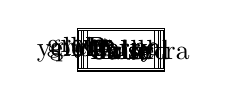
\begin{tikzpicture}[
    node/.style={%
      draw,
      rectangle,
    },
  ]

    \node [node] (A) {Ball};
    \path (A) ++(-150:\nodeDist) node [node] (B) {Color};
    \path (A) ++(-60:\nodeDist) node [node] (C) {Berry};
    \path (A) ++(-20:\nodeDist) node [node] (D) {True};
    \path (B) ++(-150:\nodeDist) node [node] (E) {Berry};
    \path (B) ++(-90:\nodeDist) node [node] (F) {False};
    \path (B) ++(-50:\nodeDist) node [node] (G) {False};
    \path (C) ++(-115:\nodeDist) node [node] (H) {True};
    \path (C) ++(-65:\nodeDist) node [node] (I) {False};
    \path (E) ++(-115:\nodeDist) node [node] (J) {True};
    \path (E) ++(-65:\nodeDist) node [node] (K) {False};


    \draw (A) -- (B) node [left,pos=0.25] {poke}(A);
    \draw (A) -- (C) node [left,pos=0.45] {great}(A);
    \draw (A) -- (D) node [right,pos=0.25] {ultra}(A);
    \draw (B) -- (E) node [left,pos=0.25] {green}(A);
    \draw (B) -- (F) node [left,pos=0.45] {yellow}(A);
    \draw (B) -- (G) node [right,pos=0.25] {red}(A);
    \draw (C) -- (H) node [left,pos=0.25] {yes}(A);
    \draw (C) -- (I) node [right,pos=0.25] {no}(A);
    \draw (E) -- (J) node [left,pos=0.25] {yes}(A);
    \draw (E) -- (K) node [right,pos=0.25] {no}(A);


\end{tikzpicture}
\\[10pt]
(f) Predicting the label in test data
\\[10pt]
Prediction for Test data number 1 is correct as the label turns out to be "YES"
\\Prediction for Test data number 2 is incorrect as the tree predicts it to be "YES", but it is mentioned as "NO"
\\Prediction for Test data number 3 is incorrect as the tree predicts it to be "YES", but it is mentioned as "NO"
\\
Thus $Accuracy = (1/3) = 0.33 \%$ 
\\[10pt]
(g) No, decision tree should not be used in the pokemon go case as it produces very little accuracy when used with the test data.
\\[10pt]
Question 3 : Recall that in the ID3 algorithm, we want to identify the best attribute that splits the examples that are relatively pure in one label. Apart from entropy, which you used in the previous question, there are other methods to measure impurity. One such impurity measure is the Gini measure, that is used in the CART family of algorithms. Solve the previous problem using the Gini Index measure.
\\[10pt]
Answer 3 :
\\[10pt] 
(a) Using the Gini index equation we can compute the values as follows:
\\[10pt]
Gini Index for label : (8/16)*(8/16)=0.25
\\[10pt]
Gini Index for "Berry" : (7/16)*(6/7 * 1/7) + (9/16)*(2/9 * 7/9) = 0.150
\\Info Gain = 1- 0.150
\\[10pt]
Gini Index for Ball: (6/16)*(1/6 * 5/6) + (7/16)*(4/7 * 3/7) = 0.159
\\Info Gain = 1- 0.159
\\[10pt]
Gini Index for Color: (3/16)*(2/3 * 1/3) + (7/16)*(3/7 * 4/7) + (6/16)*(1/2 * 1/2) = 0.242
\\Info Gain = 1- 0.242
\\[10pt]
Gini Index for Type: (6/16)*(1/2 * 1/2) + (4/16)*(1/2 * 1/2) + (4/16)*(3/4 * 1/4) = 0.203
\\Info Gain = 1- 0.203
\\[10pt]
(b) "Berry" is the root node according to Gini Index Measure as it has the highest Info Gain.
\\The two measures : Gini Index and ID3 doesn't lead to the same tree.
\\[10pt]
\textbf {2: Linear Classifiers}
\\[10pt]
Question 1 : Write a linear Classifier that correctly classifies the given dataset.
\\[10pt]
Answer 1 :
\\For the given dataset, we can define a linear classifier as: 
\\$ if $ $x3 \lor x4$ then the value is True else False
\\According to the equation $b + w1x1 + w2x2 +.....+ wnxn=0$
\\The linear classifier equation can be represented as $x3 + x4 - 0.5$
\\So the weights can be initialized as 
\\$w1=0, w2=0, w3=1, w4=1$ and bias = -0.5
\\[10pt]
Question 2 : Suppose the dataset below is an extension of the above dataset. Check if your classifier from the previous quesion correctly classifies the given dataset. Report its accuracy.
\\[10pt]
Answer 2 : 
\\According to the obtained classifier the data is correctly classified for 5 out of 7 cases.
\\The data is not classified correctly for the following cases:
\\When $x1=1, x2=1, x3=0, x4=0$ and when $x1=0 x2=0 x3=1 x4=0$
\\Thus accuracy value is 5/7 = 0.714 i.e. 71.4\%
\\[10pt]
Question 3 : Write a linear classifier that correctly classifies the given dataset.
\\[10pt]
Answer 3 : A linear classifier that correctly classifies the whole dataset:
We can observe the negative label values after combining all the three tables:
\begin{table}[h]
\centering
\caption{Negation Values}
\begin{tabular} {clclclclclc}
X1 & X2 & X3 & X4 & Label \\
  0 & 0 & 0 & 0 & -1 \\
  0 & 0 & 0 & 1 & -1 \\
  0 & 1 & 0 & 0 & -1 \\
  0 & 1 & 1 & 0 & -1 \\
  \end{tabular}
\end{table}
\\[10pt]
We observe that the values tend to be negative when $x1=0, x4=0$
\\According to the equation $b + w1x1 + w2x2 +.....+ wnxn=0$
\\The generalized equation can be stated as
$b + w1x1 + w4x4$ where $w1=1, w2=0, w3=0, w4=1$ and bias value is 0.5
\\So the final equation can be stated as: $x1 + x4 - 0.5$
\\[10pt]
\textbf {3: Experiments}
\\[40pt]
\textbf {SETTING A}
\\
1. Implementation
\\(a) The Program is Implemented using Python language.
\\For tree construction:
\\Total Data of training data file is stored in Total\_data.
\\ Features are stored in Features. 
\\Class label column is stored in class\_label\_column. 
\\Functions are created for calculating entropy and gain. 
\\Recursive calls are made to the functions to give final values for tree construction.
\\(b) The error on SettingA/training.data file is reported as 0\%. \\Accuracy is 100\% i.e. 1.0
\\(c) The error on SettingA/test.data file is reported as 0\%. \\Accuracy is 100\% i.e. 1.0
\\(d) The Maximum depth of the decision tree is 3.
\\[50pt]
2. Limiting Depth
\\(a) The Table representation:
\begin{table}[h]
\centering
\caption{Computation 2a}
\begin{tabular} {clclclclclc}
Accuracy & Depth & Standard Deviation \\
0.975928833072 & 1 & 0.0538247655494 \\
0.975928833072 & 2 & 0.0538247655494 \\
0.975928833072 & 3 & 0.0538247655494 \\
0.975928833072 & 4 & 0.0538247655494 \\
0.975928833072 & 5 & 0.0538247655494 \\
0.975928833072 & 10 & 0.0538247655494 \\
0.975928833072 & 15 & 0.0538247655494 \\
0.975928833072 & 25 & 0.0538247655494 \\
  \end{tabular}
\end{table}
\\(b) $100\%$ accuracy is reported.
\\[10pt]
\textbf {SETTING B}
\\1. Experiments
\\(a) The error on SettingB/training.data file is reported as 0\%. \\Accuracy is 100\% i.e. 1.0
\\(b) The error on SettingB/test.data file is reported as 8.57\%. \\ Accuracy is 91.4379\% i.e. 0.9143
\\(c) The error on SettingA/training.data file is reported as 0.0006\% \\Accuracy is 99.9476\% i.e. 0.9994 
\\(d) The error on SettingA/test.data file is reported as 0.0017\% \\Accuracy is 99.8353\% i.e. 0.9983
\\(e) The Maximum depth of the decision tree is 9.
\\[10pt]
2. Limiting Depth
\\(a)
\begin{table}[h]
\centering
\caption{Computation 2a}
\begin{tabular} {clclclclclc}
Accuracy & Depth & Standard Deviation \\
0.901883830455 & 1 & 0.0958846175832 \\
0.919937205651 & 2 & 0.0430400942229 \\
0.911826268969 & 3 & 0.0352830378007 \\
0.90083725798 & 4 & 0.0431774569973 \\
0.897959183673 & 5 & 0.0414454592855 \\
0.895866038723 & 10 & 0.0426245470061 \\
0.895866038723 & 15 & 0.0426245470061 \\
0.895866038723 & 25 & 0.0426245470061 \\
  \end{tabular}
\end{table}
Highest accuracy is reported for 1. So it is the best depth.
\\(b) $93.85\%$ accuracy is reported.
\\[30pt]
\textbf {SETTING C}\\
1. To handle the missing value using Method 1, the function searched for missing attribute in every row, and returned its column number. The most frequent values for the columns were then calculate using the function find unique. The missing attribute was then replaced with most frequent charachter. For Method 2, column of the missing attribute was found as in the previous. A new function calculated the most frequent attribute value and missing attribute was replaced with that class label attribute. However, due to the last minute errors, codes for these changes are not submitted.
\\2. 
\begin{table}[h]
\centering
\caption{Computation 2a}
\begin{tabular} {clclclclclc}
Accuracy & Depth & Standard Deviation \\
0.978860347492 & 1 & 0.0384691797872 \\
0.979963695505 & 2 & 0.037042433439 \\
0.98309445057 & 3 & 0.0378019577233 \\
0.98309445057 & 4 & 0.0378019577233 \\
0.98309445057 & 5 & 0.0378019577233 \\ 
0.98309445057 & 10 & 0.0378019577233 \\ 
0.98309445057 & 15 & 0.0378019577233 \\
0.98309445057 & 25 & 0.0378019577233 \\
  \end{tabular}
\end{table}
\\3. Accuracy of 100\% was acheived using the method 3 used above.
\end{document}